\documentclass[pdftex,12pt]{article}

%%% Top matter

\usepackage[usenames,dvipsnames]{color}
\usepackage[margin=1in]{geometry}
\usepackage[pdftex]{graphicx}
\usepackage[T1]{fontenc}
\usepackage{amsmath, amsthm, amsfonts}
\usepackage{amssymb, verbatim, mathpazo}
\usepackage{subfigure}
\usepackage{hyperref}

\setlength{\parindent}{0pt}
\renewcommand*\thesubfigure{(\arabic{subfigure})} 
\newcommand{\block}{\mathbb}
\newcommand{\script}{\mathcal}
\newcommand{\fancy}{\mathfrak}
\newcommand{\C}{\block{C}}
\newcommand{\R}{\block{R}}
\newcommand{\Z}{\block{Z}}
\newcommand{\Q}{\block{Q}}
\newcommand{\N}{\block{N}}
\newcommand{\I}{^{-1}}
\newcommand{\set}[2]{\{#1|#2\}}
\newcommand{\topic}[1]{\noindent{\textbf{#1}}}
\newcommand{\bij}{\longleftrightarrow}
\newcommand{\bslash}{\setminus}
\newcommand{\cl}[1]{\overline{#1}}
\newcommand{\seq}{\subseteq}
\newcommand{\ds}{\displaystyle}
\newcommand{\Wlog}{Without loss of generality }
\newcommand{\rp}{$(\Rightarrow)$ }
\newcommand{\lp}{$(\Leftarrow)$ }
\newcommand{\cbox}[2]{\fcolorbox{#1}{white}{#2}}
\newcommand{\tx}[1]{\text{#1}}
\newcommand{\horbar}{\rule{\linewidth}{0.4mm}}

\renewcommand{\qedsymbol}{\tiny$\blacksquare$}
\renewcommand{\labelenumi}{(\alph{enumi})}

\newtheorem{thm}{Theorem}
\newtheorem{prop}[thm]{Proposition}
\newtheorem{cor}[thm]{Corollary}
\newtheorem{lem}[thm]{Lemma}

\theoremstyle{definition}
\newtheorem{defn}{Definition}
\newtheorem{ex}{Example}
\newtheorem{nex}[ex]{Non-Example}

\theoremstyle{remark}
\newtheorem*{rec}{Recall}
\newtheorem*{rem}{Remark}
\newtheorem*{note}{Note}
\newtheorem*{notate}{Notation}
\newtheorem*{idea}{Idea}
\newtheorem*{question}{Question}

%%% Title

\begin{document}
\begin{center}
\horbar \\
\textsc{Julius Elinson} \hfill \textsc{\today}\\[.1cm]
\textsc{\Large{Image-Based Rock-Climbing Simulator}}\\[-.1cm]
\horbar \\[.4cm]
\end{center}

%%% Body
\subsection*{Background}
Rock-climbing is a sport that presents both a physical and athletic challenge. At indoor gyms, climbing walls contain a number routes with varying difficultly that are typically delimited by the color of the grips. The difficulty is determined by the number of grips, their sizes and positions, as well as contours in the wall itself. To complete a route, a person must use only the designated grips with his/her hands and feet to ascend to the top; the goal is simply to get to the last grip and thus a climber can use any subset of the available grips and in any order. Thus a route is a set of grips, whereas a path, or solution, is a ordered list of tuples of grips, where each tuple represents the positions of each limb at any given position. Climbing requires both the physical stamina to ascend the wall, but also constructing a viable path where one's body weight is balanced and each move can be completed the physical constraints of the body.

\subsection*{Objectives}
The goal of this project was to simulate a rock climber by generating a physically-feasible path to solve a route based on an input image. As part of that objective, the program had to be able to identify a particular route within an image, analyze each grip in the route, model basic human motion and perform an intelligent search to find a path to the top. To limit the scope and difficulty of the project, only routes without overhang\footnote{A overhang is when a wall juts out so that climbing it would cause the climber to become supine.} were considered, so that motion and forces would be limited to the 2-D plane. \\ \\
In order to simulate a human interacting with grips, the program had to be able to analyze a wide array of grip types. Different grips at different orientations can support different forces applied on them. Moreover, variations in size, texture and shape have implications for what and how many limbs can be put on a particular grip at a given time. Additionally, analyzing a climber's position required considering each limb in the context of the others in order to respect physical constraints of the human body, as well as analyze forces and weight distribution in the aggregate. \\ \\ 
The search algorithm had to account for the physical implications of a possible path. While a shortest path offers certain advantages, the number of moves also had to weighed against the physical strain induced by each move.

\subsection*{Implementation}
\subsubsection*{Tools}
The program is named jug, after a type of hand-grip that is very easy to grab and apply weight to. 
Jug was developed in C++ using both Qt \& OpenCV. Qt provides a number of convenience classes for streamlined development and OpenCV is an excellent library for image processing and provides some basic graphical user interface support. The program is cross-platform and uses CMake for the build process.

\subsubsection*{Image Processing}
Jug comes with several example climbing wall images and it can load user-specified files. The program starts by prompting the user to select a grip with their mouse that is contained in the route they wish to solve. Using this, the RGB image is first converted to HSV space. The reason for this is that hue is generally more invariant between shades of the same color then in the entire RGB space. Grips are often different shades of the same color or have white tints from chalk residue and this helps mitigate the effect of that. The hue value of the pixel selection by the user is then used to threshold the entire image using a small tolerance range.\\ \\
The result of thresholding is a binary image that is noisy, as there are often holes in regions or small speckles of white pixels that do not correspond to interesting regions. To correct this, an erosion and dilation algorithm is used. In this process, the perimeter of any region is eroded several pixels and then expanded for twice as many pixels, and finally eroded once again. For small white speckles, the first erosion process will remove the region entirely so that it will disappear and hence not be dilated. For holes within regions, the dilation process will cause the hole to fill and then there will be no perimeter there when the erosion occurs again. For all the other regions, the net effect of the three steps is no change. The contour of each remaining region in the binary image is used to represent a grip.

\subsubsection*{Grip Analysis}
Using the grip contour, a number of intrinsic properties of the grip are determined. The area, perimeter, and center of mass are all computed, as well as several more complex representations. One such calculation is of the grip's convexity defects, which is performed by analyzing the gaps between the contour and its convex hull. This yields the number of such defects as well as their sizes and relative locations.\\ \\
Additionally, to analyze the grip's orientation, the program computes what I refer to as the normal field. This is a tally of the different normal vectors along the contour. Because the contour is a contiguous, 8-connected\footnote{Pixels are 8-connected if all 8 surrounding pixels, including diagonals, are considered neighbors.} discrete set of pixels, the normal vectors are computed on each pixel by computing the line orthogonal to the vector connecting the previous and next pixels. From this construction there are only a small set of possible orientations. Ultimately the normal field tries to capture the relative sizes of the grip sides in each direction.

\subsubsection*{Physical Engine}
In jug, a human is modeled as 4 limbs (two arms, two legs) and a center of mass. Half the climber's weight is in the center and the other half is distributed evenly over each limb. The forces are computed at the center of mass such that an arm extending diagonally out and down will contribute both a horizontal and vertical force.\\ \\
The feasibility of a position, which is a ordered list of 4 grips representing the locations of the limbs, is determined by both analyzing the forces, as well as simpler binary criteria. These criteria sanity check the climber's position and filter out anything that is unrealistic. The checks for this ensure the following is true about a position:
\begin{itemize}
\setlength{\itemsep}{0pt}
\setlength{\parskip}{0pt}
 \item each limb is both within and at least certain distances from the center of mass;
 \item the corresponding right and left limbs are not significantly crossed-over;
 \item the climber's feet are always below at least one hand;
 \item the grips that the hands are on can in fact support hands;\footnote{A number of grips are small numbs that realistically only provide a foot support because they are too small to wrap any number of fingers around.}
 \item if a position has multiple limbs on a single grip, that grip can support that many limbs at once.
\end{itemize}
The last two criteria are determined by analyzing the perimeter and area of the grips.\\ \\
Once the position has been determined to be reasonable, the forces are analyzed by computing how much weight each grip can support. To do this, the angle at which the limb is approaching the grip is necessary. This angle is then used to look-up the corresponding slope in the normal field of the grip. This value is then scaled by a function of the area and perimeter, as proxies for the grip's depth and general quality. The resulting value then scales the directional vector to produce a vector force. The forces are summed across all grips. If the support from the grips counterbalances the force of gravity, the position is deemed feasible.

\subsection*{Path Search}
There are three components of the search algorithm: determining a start position, expanding a state's neighbors, and the search itself. In rock climbing, a route's start position is specified by labeling where the hands begin, usually with a tag or marker. Instead of doing additional image processing to find this, the program searches over possible start positions somewhat naively. It looks at the four lowest grips and checks the feasibility of permuting each limb and in some cases sharing grips between limbs. This will continue by considering the set of the next four lowest grips until a feasible position is found.\\ \\
Each move is assumed to change the position of a single limb at a time. Thus the neighbors are naively generated by considering moving each limb to each grip. The branching factor is further increased because the center of mass is not determined uniquely by a set of 4 grips. In order to capture the joints in human limbs that allow them to extend or contract within a certain range, the center of mass must be allowed to differ from the geometric center. The set of possible centers can be defined as the intersection between the tori made by considering the minimum and maximize distances a limb needs to be from the center. Since this is computational intensive to compute and the precision of knowing each pixel would be excessive for the purposes of the problem, a lattice of points is sampled centered around the geometric center.\\ \\
Although the problem lends itself to heuristic search, only breadth first search was in fact implemented, and therefore the program determines the route with the fewest moves. As the results demonstrated, other parts of the program needed finer tuning before the utility of A$^*$ could be realized.
\subsection*{Results}
Example routes and the corresponding solutions, if any were found, are shown in Fig.~\eqref{fig:pink0} - \eqref{fig:fail}. For all solution paths, positions are label by highlighting the contours of where each of the four limbs are. The legend is as follows:

\begin{itemize}
 \item Blue -- Left foot
 \item White -- Right foot
 \item Red -- Left hand
 \item Green -- Right hand
 \item Black circle -- Center of mass
 \item If two limbs are sharing a grip, which is called ``matching'', only one color will be drawn. These cases are marked in each figure.
\end{itemize}

\subsubsection*{Examples}
In Fig.~\eqref{fig:pink0}, the start position in panel 1 is a logical one. The hands are matched on a large grip which is in fact the actual designated start grip. Panel 2 shows an issue with limbs being too close together; a person would not be able to fit in that small of a space. Moving from panel 2 to panel 3 is a very large and impractical move. The position in panel 5 and 6 would be difficult to maintain and does not reflect accurate weight balancing.\\ \\
In Fig.~\eqref{fig:pink2}, the start again is a logical one and uses the designated start grip. Moves 2, 3, and 4 are all good ones and demonstrate good climbing technique. Panel 5 shows the climber confined to a small position. However, moving from 5 to 6 is a very good move. Although the next grip is slightly to the right, the climber grabs it with their left hand because the cross-over is tolerable and then the climber is in a much better position to advance because the right hand is free to reach out, as it does in panel 7. Panel 9, though, does not demonstrate effective force balancing. A better path would have been moving the left foot to the small grip near the center of the image and bringing the right foot up using the small red grips to the right.\\ \\
In Fig.~\eqref{fig:pink3}, the start position is not ideal: the hands are matched on the small triangular grip when at least one hand should be on the longer one that it then moves to. Panel 2 shows the climber with his/her limbs too close together. The moves in 3-6 are all reasonable; however there are fewer grips visible in this route and thus the climber could finish the route only so many ways. \\ \\
In Fig.~\eqref{fig:fail}, the program could not properly determine where the grips were and consequently could not formulate a path to solve any of the routes.

\subsubsection*{Analysis}
Overall jug understands how to formulate reasonable paths. It demonstrates certain techniques such as moving one type of limb and bringing the other limb of that type to match it. It has foresight to not get itself tangled by moving the wrong hand. It knows to favor larger grips over smaller ones.\\ \\
However, the program has a number of shortcomings. Perhaps most notably is its sense of size. Although the constants that make up the climber's specifications were tuned, there is no size normalization step. Because the photos give no sense of how large, an absolute sense, each grip and move is, there is no currently no way to calibrate the climber's dimensions to the specific image. This contributed to why the climber could make long reaches and also fit in small spaces: the constants limiting this behavior had to be relaxed so that any solution at all could be found for more than one specific input image.\\ \\
The program also does not have a meaningful sense of forces. Although it does force analysis, rarely was an imbalance in forces a limiting factor in its search, and moreover a number of positions did not reflect accurate physics. The weights that translate physical properties into a force vector need to be fined-tuned, if not machine learned. The difficulty with doing this is that there is not always a clear-cut correct solution that could be used for training in some supervised learning algorithm. \\ \\
Additionally, the image processing is still not robust as it could be. Particularly in the last example, because the entire image is dark and the grip colors are all subdued, detecting routes by hue is not effective. The detection could be improved by filtering grip candidates by checking the RGB difference from the selected grip and the candidate. Furthermore, edge detection could be used to first identify all grips and the hue thresholding could be applied afterwards, to better capture entire grips, rather than sometimes just part of one.

\begin{figure}
 \centering
 \subfigure[Hands matched at green]
 {\includegraphics[width=.3\textwidth]{../../img/output/pink/move_0.jpg}} \hspace{2pt}
  \subfigure[Feet match at white]
 {\includegraphics[width=.3\textwidth]{../../img/output/pink/move_1.jpg}} \hspace{2pt}
 \subfigure[Right hand reaches up]
 {\includegraphics[width=.3\textwidth]{../../img/output/pink/move_2.jpg}} \hspace{2pt} 
 \subfigure[Hands match at green]
 {\includegraphics[width=.3\textwidth]{../../img/output/pink/move_3.jpg}} \hspace{2pt} 
 \subfigure[Left foot moves out]
 {\includegraphics[width=.3\textwidth]{../../img/output/pink/move_4.jpg}} \hspace{2pt} 
 \subfigure[Right foot moves up]
 {\includegraphics[width=.3\textwidth]{../../img/output/pink/move_5.jpg}} \hspace{2pt} 
 \subfigure[Left hand grabs last grip]
 {\includegraphics[width=.3\textwidth]{../../img/output/pink/move_6.jpg}} \hspace{2pt} 
 \caption{Solution to pink course. Throughout, the white outline marks the right foot, the blue marks the left foot, the red marks the left hand, and green marks the right hand. The exceptions are when limbs share a grip (``match''), in which case only one color is drawn. The black circle is the center of mass.}
 \label{fig:pink0}
\end{figure}


\begin{figure}
 \centering
 \subfigure[Hands matched at green]
 {\includegraphics[width=.3\textwidth]{../../img/output/pink2/move_0.jpg}} \hspace{2pt}
  \subfigure[Left hand up]
 {\includegraphics[width=.3\textwidth]{../../img/output/pink2/move_1.jpg}} \hspace{2pt}
 \subfigure[Right hand matches at green]
 {\includegraphics[width=.3\textwidth]{../../img/output/pink2/move_2.jpg}} \hspace{2pt} 
 \subfigure[Right foot up]
 {\includegraphics[width=.3\textwidth]{../../img/output/pink2/move_3.jpg}} \hspace{2pt} 
 \subfigure[Left foot matches at white]
 {\includegraphics[width=.3\textwidth]{../../img/output/pink2/move_4.jpg}} \hspace{2pt} 
 \subfigure[Left hand up (above green)]
 {\includegraphics[width=.3\textwidth]{../../img/output/pink2/move_5.jpg}} \hspace{2pt} 
 \subfigure[Right hand reaches right]
 {\includegraphics[width=.3\textwidth]{../../img/output/pink2/move_6.jpg}} \hspace{2pt} 
 \subfigure[Left foot up]
 {\includegraphics[width=.3\textwidth]{../../img/output/pink2/move_7.jpg}} \hspace{2pt} 
 \subfigure[Feet match at white]
 {\includegraphics[width=.3\textwidth]{../../img/output/pink2/move_8.jpg}} \hspace{2pt} 
 %\subfigure[Left hand grabs last grip]
 %{\includegraphics[width=.3\textwidth]{../../img/output/pink2/move_9.jpg}} \hspace{2pt} 
 \caption{Solution to red route. The last move, left hand up to the top, is omitted for space. See Fig.~\eqref{fig:pink0} for the legend.}
 \label{fig:pink2}
\end{figure}

\begin{figure}
 \centering
 \subfigure[Hands matched at green]
 {\includegraphics[width=.3\textwidth]{../../img/output/pink3/move_0.jpg}} \hspace{2pt}
  \subfigure[Left foot up]
 {\includegraphics[width=.3\textwidth]{../../img/output/pink3/move_1.jpg}} \hspace{2pt}
 \subfigure[Left hand up]
 {\includegraphics[width=.3\textwidth]{../../img/output/pink3/move_2.jpg}} \hspace{2pt} 
 \subfigure[Right hand matches at green]
 {\includegraphics[width=.3\textwidth]{../../img/output/pink3/move_3.jpg}} \hspace{2pt} 
 \subfigure[Right food up]
 {\includegraphics[width=.3\textwidth]{../../img/output/pink3/move_4.jpg}} \hspace{2pt} 
 \subfigure[Left hand up (grip interior)]
 {\includegraphics[width=.3\textwidth]{../../img/output/pink3/move_5.jpg}} \hspace{2pt} 
 \caption{Solution to the pink route. See Fig.~\eqref{fig:pink0} for the legend.}
 \label{fig:pink3}
\end{figure}

\begin{figure}
 \centering
 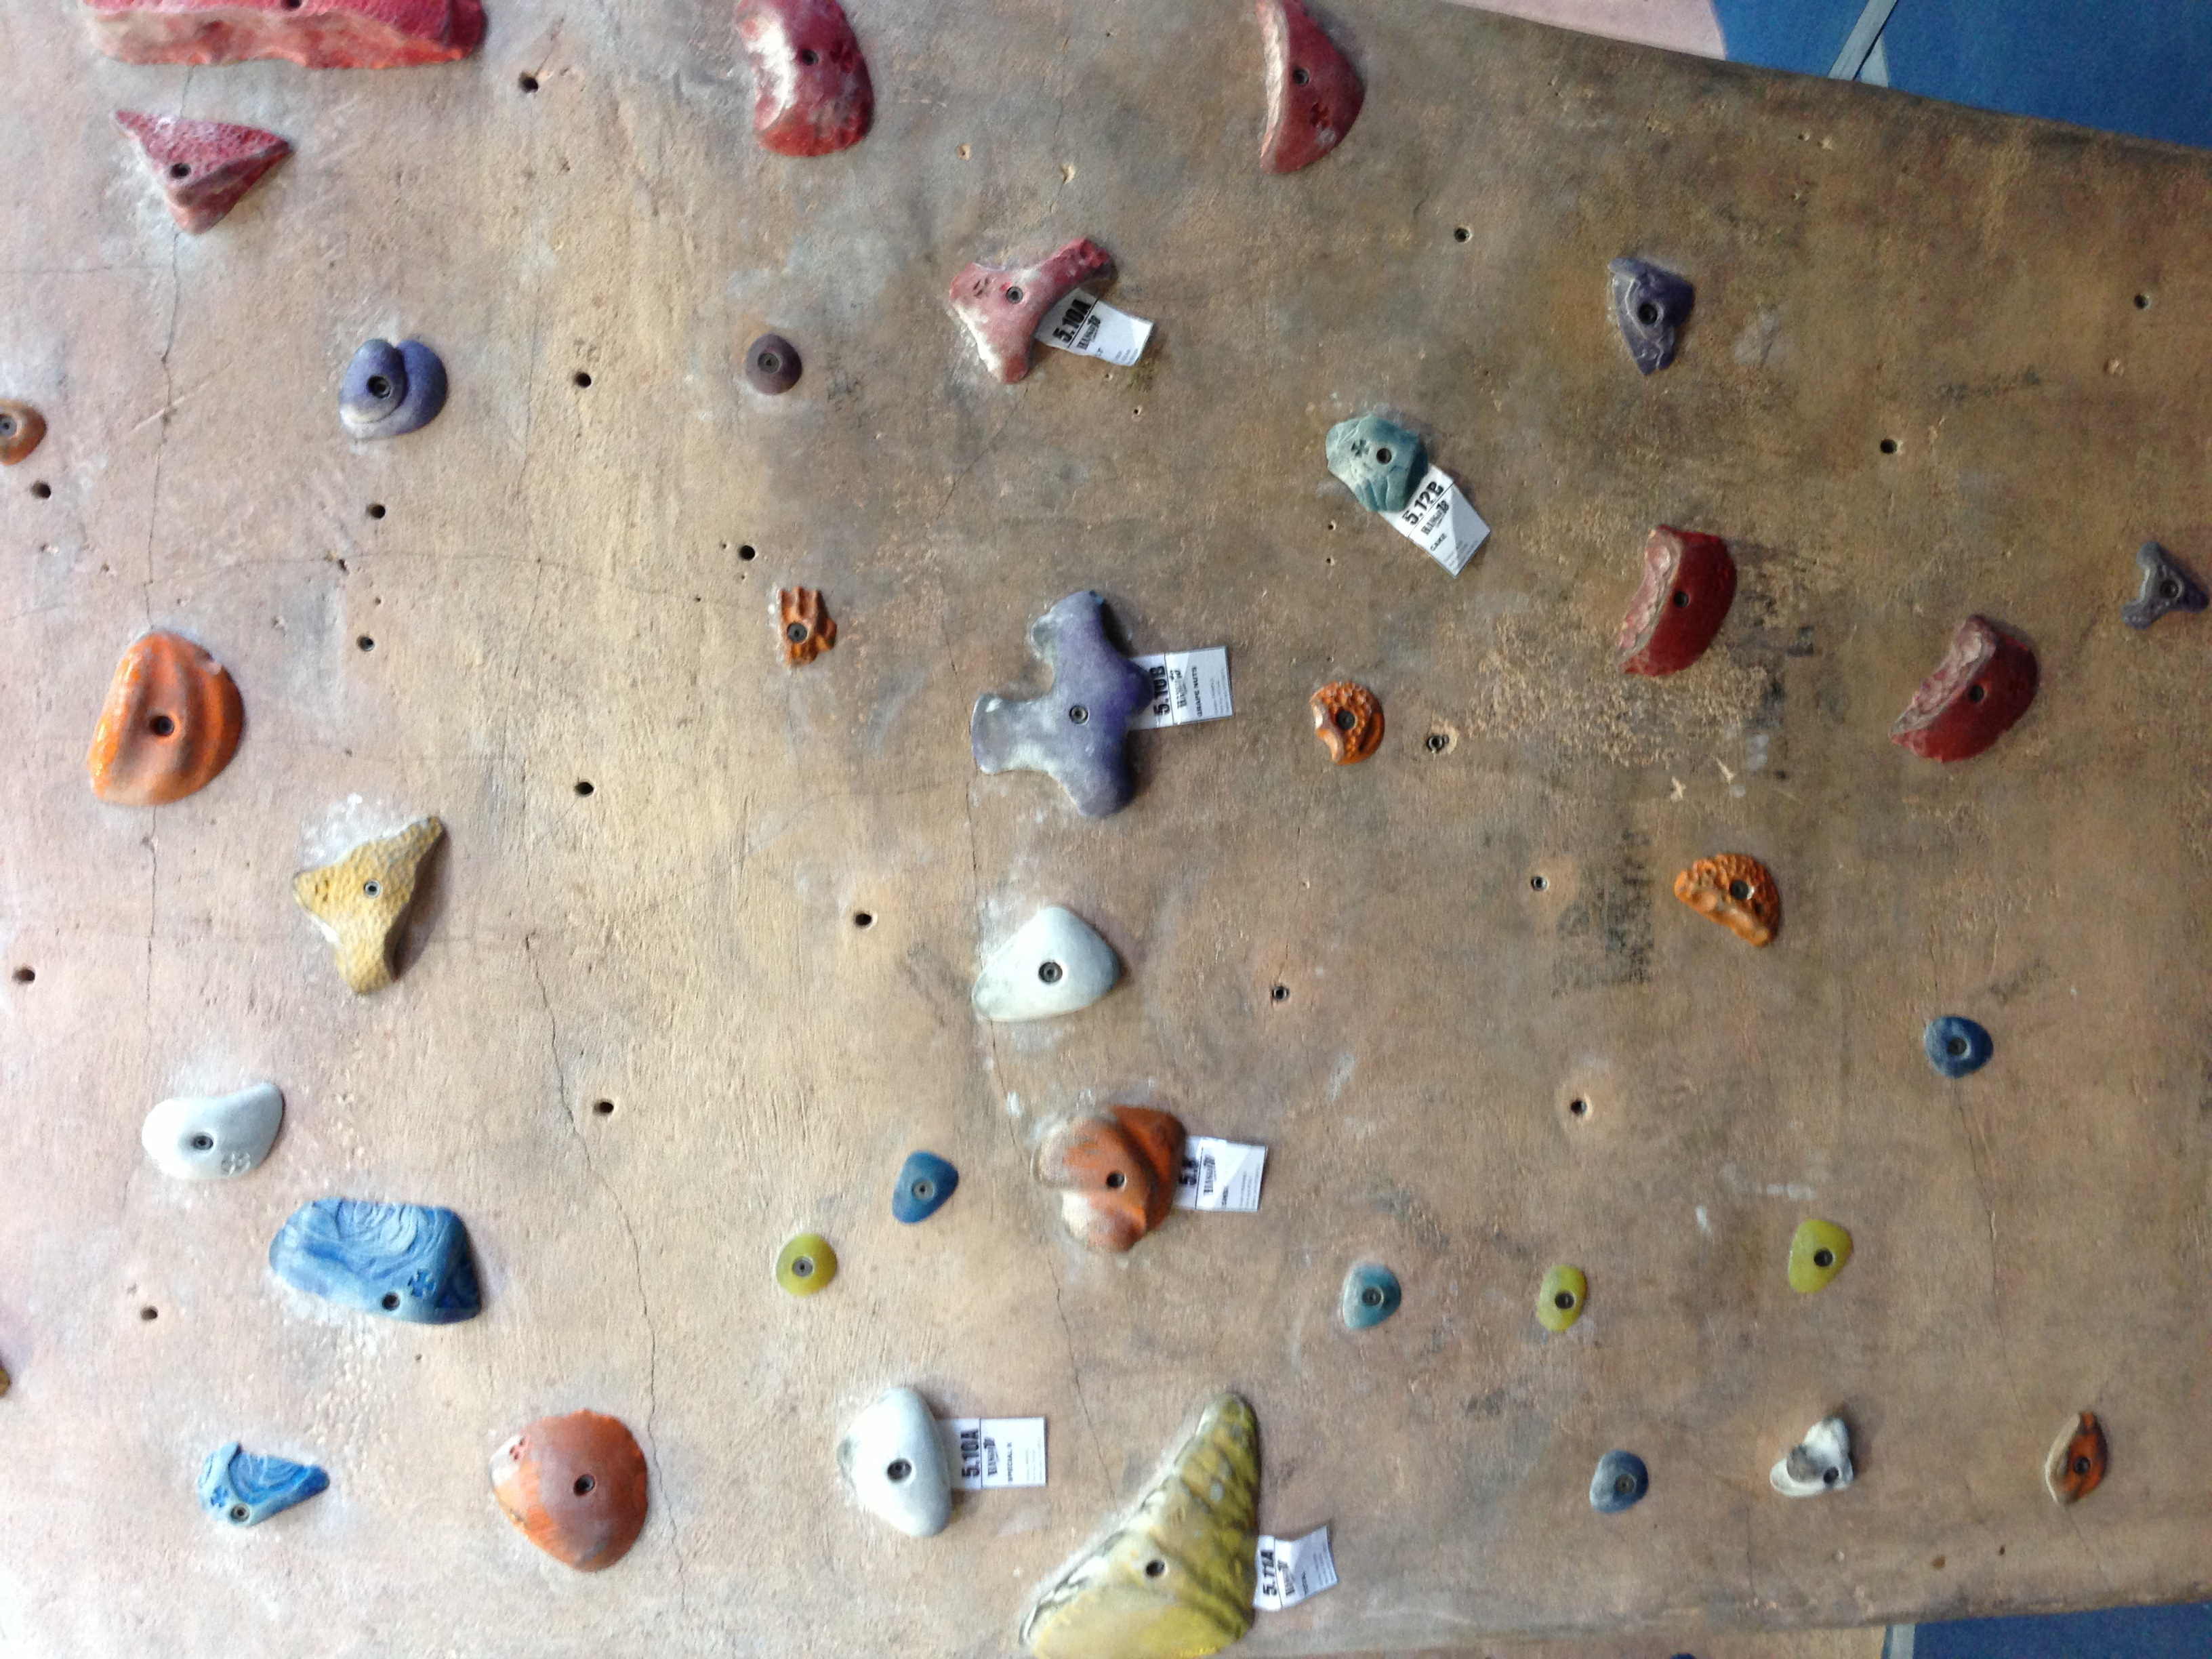
\includegraphics[angle=-90,width=.6\textwidth]{../../img/input/test3.jpg}
 \caption{For all routes in this photo, the program was unable to find a solution.}
 \label{fig:fail}
\end{figure}



\end{document}